Les \gls{bdd} sont des outils permettant de stocker et retrouver des \glspl{data}, c'est à dire des valeurs brutes. Ces outils se trouvent au coeur des \glspl{si}, et sont donc indispensables aux entreprises.

En informatique, les bases de données sont informatisée, définies et manipulées grâce à des logiciels nommés \glspl{sgbd}.

Il existe différents types de bases de données, mais le marché reste dominé par les \glspl{bddr} \footnote{\label{part_de_marché_relationnel}Classement des \glspl{sgbd} les plus populaires : \url{http://db-engines.com/en/ranking}}. Ces dernières sont gérées par des SGBD relationnels. Parmi les plus connus, on trouve :
\begin{itemize}
\item Oracle,
\item MySQL,
\item PostgreSQL.\\
\end{itemize}

Ces logiciels proposent tous de définir et de manipuler des bases de données par le biais du \gls{sql}, un langage déclaratif et normé, implémenté par les SGBD avec des écarts vis à vis de ce que préconise la norme\footnote{\label{differences_implementation_sql_sqgbd}Comparer les documentations Oracle et MySQL pour modifier une table \url{https://docs.oracle.com/cd/B28359_01/server.111/b28286/statements_3001.htm} contre \url{https://dev.mysql.com/doc/refman/5.7/en/alter-table.html}}. De ce fait, deux SGBD distincts ne proposent pas \textit{exactement} le même SQL.

Cela amène la problématique suivante : les bases de données relationnelles sont presques incontournables, et ne peuvent être utilisées qu'en ayant connaissance du langage SQL, ce dernier variant selon le SGBD choisi. 

Ce projet propose une application permettant de manipuler une base de données relationnelle \textit{sans} avoir recours au SQL et sur n'importe quel SGBD.

La figure \ref{sans_idb_schema} illustre l'utilisation habituelle des SGBD.

La figure \ref{avec_idb_schema} illustre l'utilisation d'un SGBD avec l'application.

\begin{figure}[!h]
  \centering
  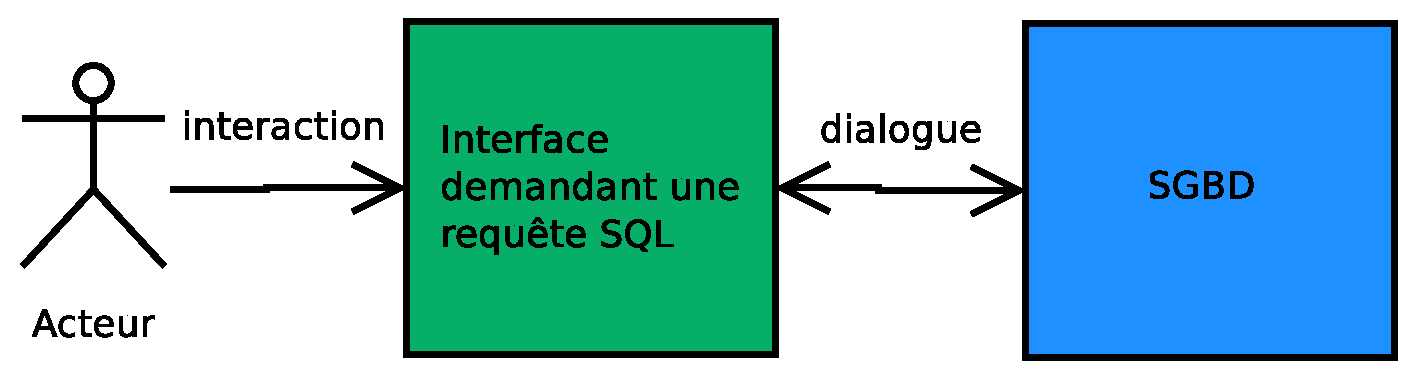
\includegraphics[width=14cm]{images/sans_idb.eps}
  \caption{Utilisation classique d'un SGBD.}
  \label{sans_idb_schema}
\end{figure}

\begin{figure}[!h]
  \centering
  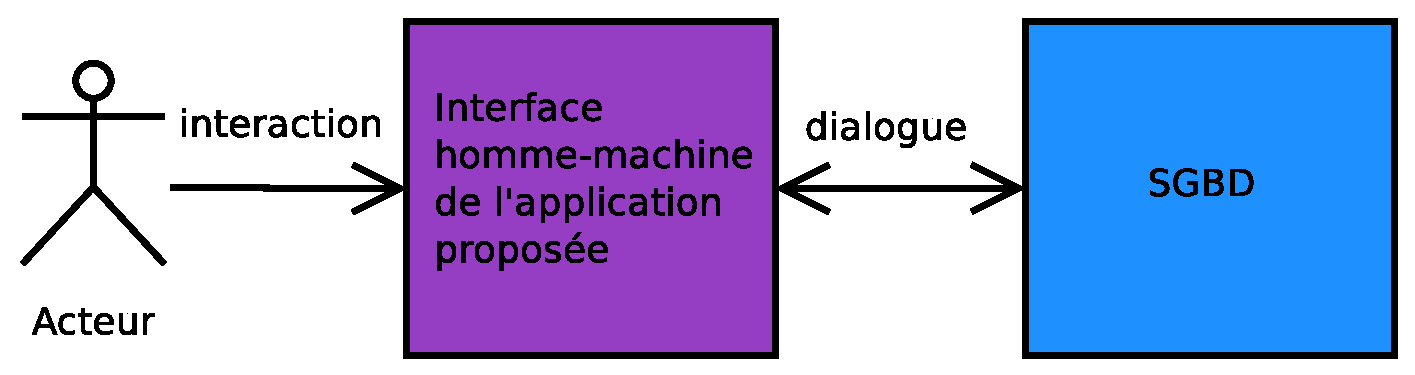
\includegraphics[width=14cm]{images/avec_idb.eps}
  \caption{Utilisation d'un SGBD avec l'application du projet.}
  \label{avec_idb_schema}
\end{figure}
%TODO : donner un nom à l'application
